\documentclass{article}

\usepackage[utf8]{inputenc}

\usepackage{amsmath, bm}
\usepackage{graphicx}
\usepackage{amssymb}
\usepackage{float}
\usepackage{caption}
\usepackage{subcaption}
\usepackage{hyperref}
\usepackage{tikz}
\usepackage{layout}

\usepackage[margin=1in]{geometry}
\usepackage{listings}
\usepackage{xcolor}
\usepackage{color, colortbl}
\usepackage{textgreek}
\usepackage{mathrsfs}
\usepackage{savetrees}

\usetikzlibrary{calc}
\usetikzlibrary{angles,quotes} % for pic
\usetikzlibrary{patterns,snakes}
\usetikzlibrary{arrows}
\tikzset{>=latex} % for LaTeX arrow head

\setlength{\parskip}{\baselineskip}%
\setlength{\parindent}{0pt}%
\linespread{0.9}


\definecolor{codegreen}{rgb}{0,0.6,0}
\definecolor{codegray}{rgb}{0.5,0.5,0.5}
\definecolor{codepurple}{rgb}{0.58,0,0.82}
\definecolor{backcolour}{rgb}{0.95,0.95,0.92}

\lstdefinestyle{mystyle}{
    backgroundcolor=\color{backcolour},   
    commentstyle=\color{codegreen},
    keywordstyle=\color{magenta},
    numberstyle=\tiny\color{codegray},
    stringstyle=\color{codepurple},
    basicstyle=\ttfamily\footnotesize,
    breakatwhitespace=false,         
    breaklines=true,                 
    captionpos=b,                    
    keepspaces=true,                 
    numbers=left,                    
    numbersep=5pt,                  
    showspaces=false,                
    showstringspaces=false,
    showtabs=false,                  
    tabsize=2
}

\lstset{style=mystyle}



\begin{document}

\title{GA3: Heat Exchanger Interim Report}
\author{lwp26}
\date{May 2024}
\maketitle 

\iffalse
\begin{abstract}
    \centering
    This report presents the development of a software tool to help solve constrained design optimization of a shell and tube heat exchanger.
    The software is developed in Python and uses LMTD and NTU methods to solve for the output parameters.
    Computational model is compared with experimental data 
    Various optimization algorithms were tested with constraints and the results are presented.
\end{abstract}
\fi

%-----------------------------------------------------------------------------------------
\section{Introduction}
%-----------------------------------------------------------------------------------------

Heat exchangers have a wide range of applications in HVAC, power generation and chemical industries.
These essential components are typically much larger than other components in a system and can significantly contribute to the overall cost.
Designing high performance, low cost heat exchangers involves solving complex optimization problems with multiple constraints.
This report presents the development of a software tool to help solve constrained design optimization of a shell and tube heat exchanger.
The software is developed in Python and uses LMTD and NTU methods to solve for the output parameters.
Computational model is compared with experimental data gathered from a heat exchanger test rig, from which the uncertainty is quantified.
Simplicial homology global optimization algorithms are tested with constraints and the results are presented.

% Various optimization algorithms were tested with constraints and results are presented.
 
\subsection{Objectives}
% list the objectives of the experiment

\begin{itemize}
    \item To analyse pressure loss and heat transfer for various shell and tube heat exchanger designs.
    \item To produce a software tool for constrained design optimization of shell and tube heat exchangers.
    \item To select an optimal design to be compared with other groups designs and software tools.
    \item To manufacture and test the selected design against other groups and software predictions.
\end{itemize}

\subsection{Background}
% brief overview of heat exchangers and the experiment
% Compare Kerns, Bell-Delaware and Tinker methods for pressure drop calculations
One of the key challenges in heat exchanger design is the accurate prediction of shell-side pressure drop and heat transfer coefficients.
Two methods commonly used in industry are Kerns and Bell-Delaware methods.
Kerns method is often used for preliminary design calculations, while the Bell-Delaware method is widely used for detailed design.
The 

% analyse mechanical systems

\section{Performance Characterisation}

\subsection{Hydraulic Analysis}

% Brief overview of pressure drop of various components
% Correction made to baffles
% Fit empirical calculations to experimental data
The pressure drop across for each section of the heat exchanger can be calculated from the mass flow rate and the geometry of the components through empirical relations.
The compressor characteristics in the closed loop circuit relate the equivilent pressure drop for a given mass flow rate.
This is iteratively solved to calculate the mass flow rate for a heat exchanger design and compressor characteristic.

The pressure drop in shell side flow is more complex than the tube side flow due to bundle pass and baffle configurations.
Kerns method was used to calculate the pressure drop in each cold flow pass.
This uses an effective diameter which depends on triangular or square pitch and a bundle crossflow area, $A_s$ defined by equation 6 in the handout \cite{handout}.

\begin{equation}
  d'_{\text{sh,sq}} = \frac{4(Y^2 - \pi d_o^2/4)}{\pi d_o / 2}  \quad \text{,} \quad d'_{\text{sh,tri}} = \frac{4 \left( \frac{Y^2 \sqrt{3}}{4} - \frac{\pi d_o^2}{8} \right)}{\pi d_o / 2}
\end{equation}

The shell velocity and pressure drop for 1 of $N_b$ cold stages with $n_b$ baffles is given by the equations below \cite{HE_design}.
\begin{equation}
  v_\text{sh} = \frac{\dot{m}_1}{N_b A_s} \quad \text{and} \quad \Delta P = \frac{1}{2}f \rho v_\text{sh}^2 \left( \frac{d_\text{sh}}{d'_\text{sh}} \right) (n_b + 1)
\end{equation}
Where the friction factor $f$ is calculated from the effective diameter Reynolds number $f = 0.202 \times Re_{d'_\text{sh}}^{-0.153}$. \\
The hot side pressure drop is similar way to the worked example handout \cite{worked_example} with some minor modifications for $N_t$ hot passes.
The pressure loss factors $K_c$ and $K_e$ depend on $\sigma$ which is the ratio of a single stage tube area to the expansion area.
For multipass configurations with constrictions into, and expansions out of U bends have twice the area of a single pass.
The pressure loss coefficient in the sharp U bends was estimated to be 1.0 for each bend on both the hot and cold sides.

% Basically we used kerns method when we should have used tinker method
% Turbulent flow is obtained at lower Reynolds numbers on the shell side.

\subsection{Conductivity}

The Nusselt numbers and heat transfer coefficients are calculated in the same way as the worked example, but for each hot pass.
The total conductivity is the sum of the conductivities over all hot passes

\subsection{$\mathcal{E}$-NTU}
% read up on this
% Fscale for various arrangements
The $\mathcal{E}$-NTU method is used to calculate the heat transfer rate for a wide range of heat exchanger configurations.
The effectiveness can be found from a dimensionless number of "transfer units" denoted $NTU$ and a heat capacity rate ratio, $C^*$ or $R$.
\begin{equation}
  NTU = \frac{HA}{C_{\text{min}}} \quad \text{and} \quad C^* = \frac{C_{\text{min}}}{C_{\text{max}}} = \frac{(\dot{m}c_p)_{\text{min}}}{(\dot{m}c_p)_{\text{max}}}
\end{equation}
The $\mathcal{E}$-NTU method changes when the shell fluid is minimum or maximum heat capacity rate.
A generalised method known as P-NTU defines a temperature effectiveness $P$ as a function of NTU and a ratio of heat capacity rates $R$ both defined below.
\begin{equation}
   R_1 = \frac{C_1}{C_2} \quad \quad P_1 = \frac{C_\text{min}}{C_1} \mathcal{E} = f(NTU, R_1)
\end{equation}
Extensive work has been done to find functions, $f$, for various heat exchanger configurations to calculate $P$, and hence $\mathcal{E}$ \cite{HeatTransfer}.
This can then used to obtain outlet temperatures and heat transfer rate $\dot{Q}$.


\subsection{LMTD}
% read up on this

The Log Mean Temperature Difference (LMTD) method is based on the analytical solution for a single stage counterflow heat exchanger.
For a general heat exchanger, a correction factor $F$ is applied which represents the deviation from counterflow log mean temperature difference.

\begin{equation}
  \dot{Q} = HAF \Delta T_{\text{lm}} \quad \text{where} \quad \Delta T_{\text{lm}} = \frac{\Delta T_1 - \Delta T_2}{\ln(\Delta T_1 / \Delta T_2)}
\end{equation}
For this counterflow definition of F, $\Delta T_1 = T_{\text{hot,in}} - T_{\text{cold,out}}$ and $\Delta T_2 = T_{\text{hot,out}} - T_{\text{cold,in}}$.
Variations from this, including the coflow case or multiple passes, require the F factor to be calculated from the P-NTU temperature effectiveness, $P_1$, and heat capacity rate ratio $R_1$
from well defined relations \cite{HeatTransfer}.


\subsection{Comparison of Methods and Experimental Data}

Experimental data for previous designs was compared with our model to improve the accuracy.

\subsubsection{Hydraulic Analysis}

\begin{figure}[H]
  \centering
  \begin{subfigure}{.49\textwidth}
    \centering
    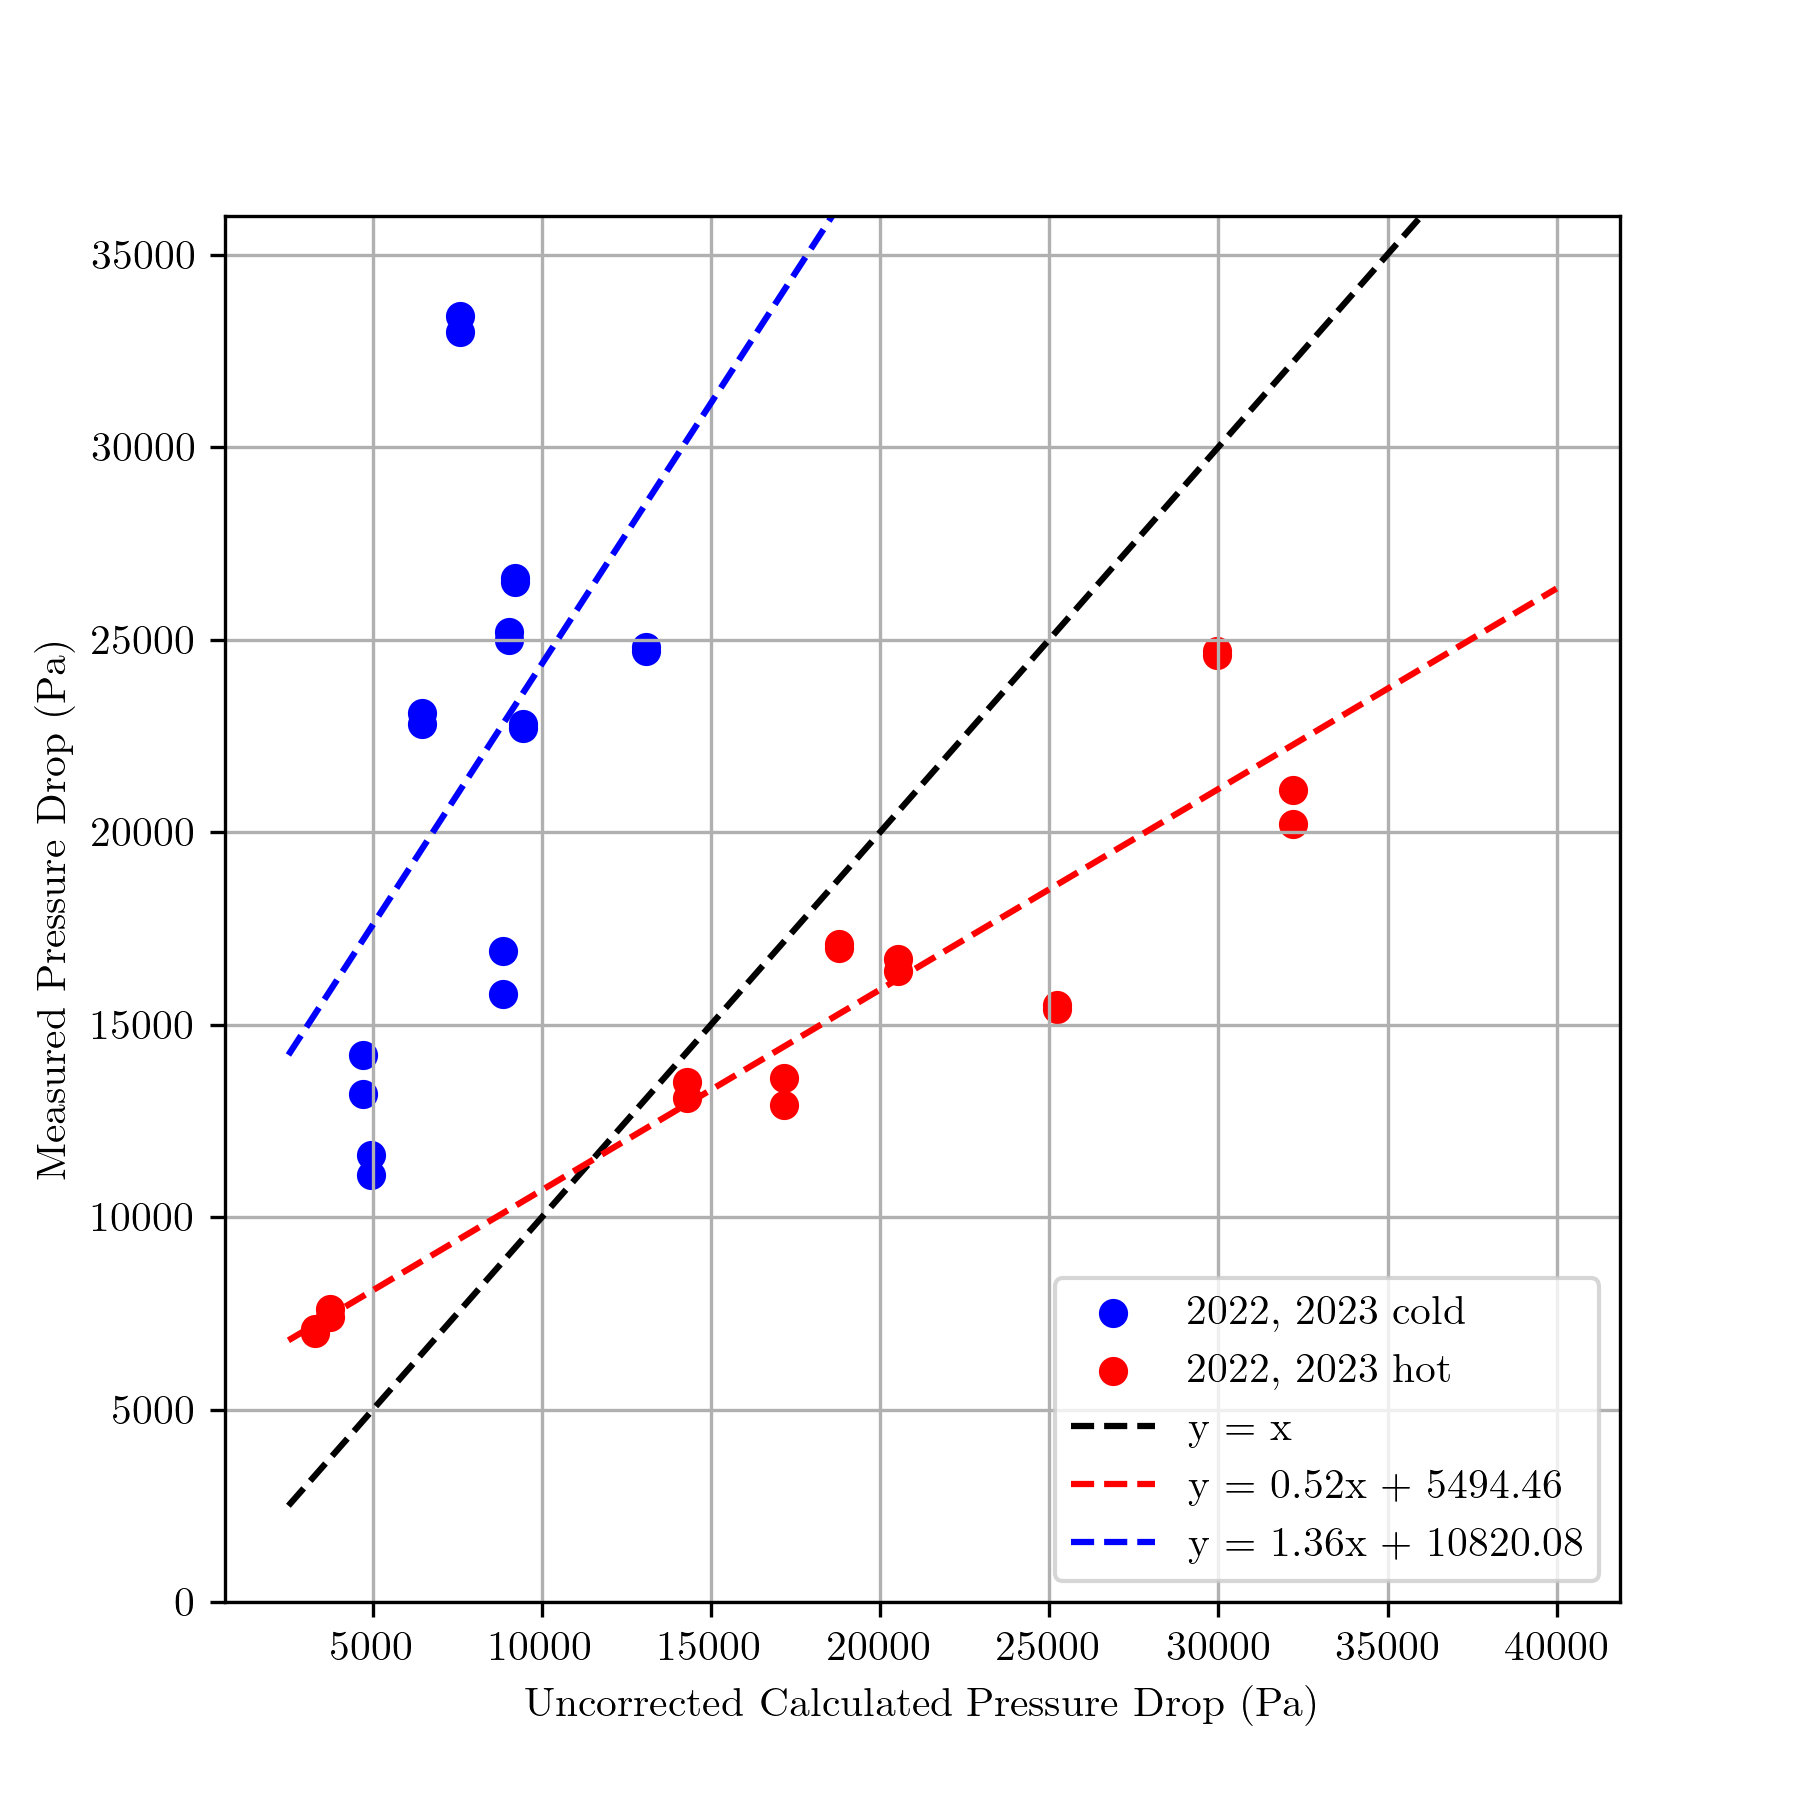
\includegraphics[width=0.99\textwidth]{dp_ucalc_vs_meas.png}
    \caption{Correction lines from 2022 and 2023 designs.}
    \label{fig:uncorrected_pressure_drops}
  \end{subfigure}
  \begin{subfigure}{.49\textwidth}
    \centering
    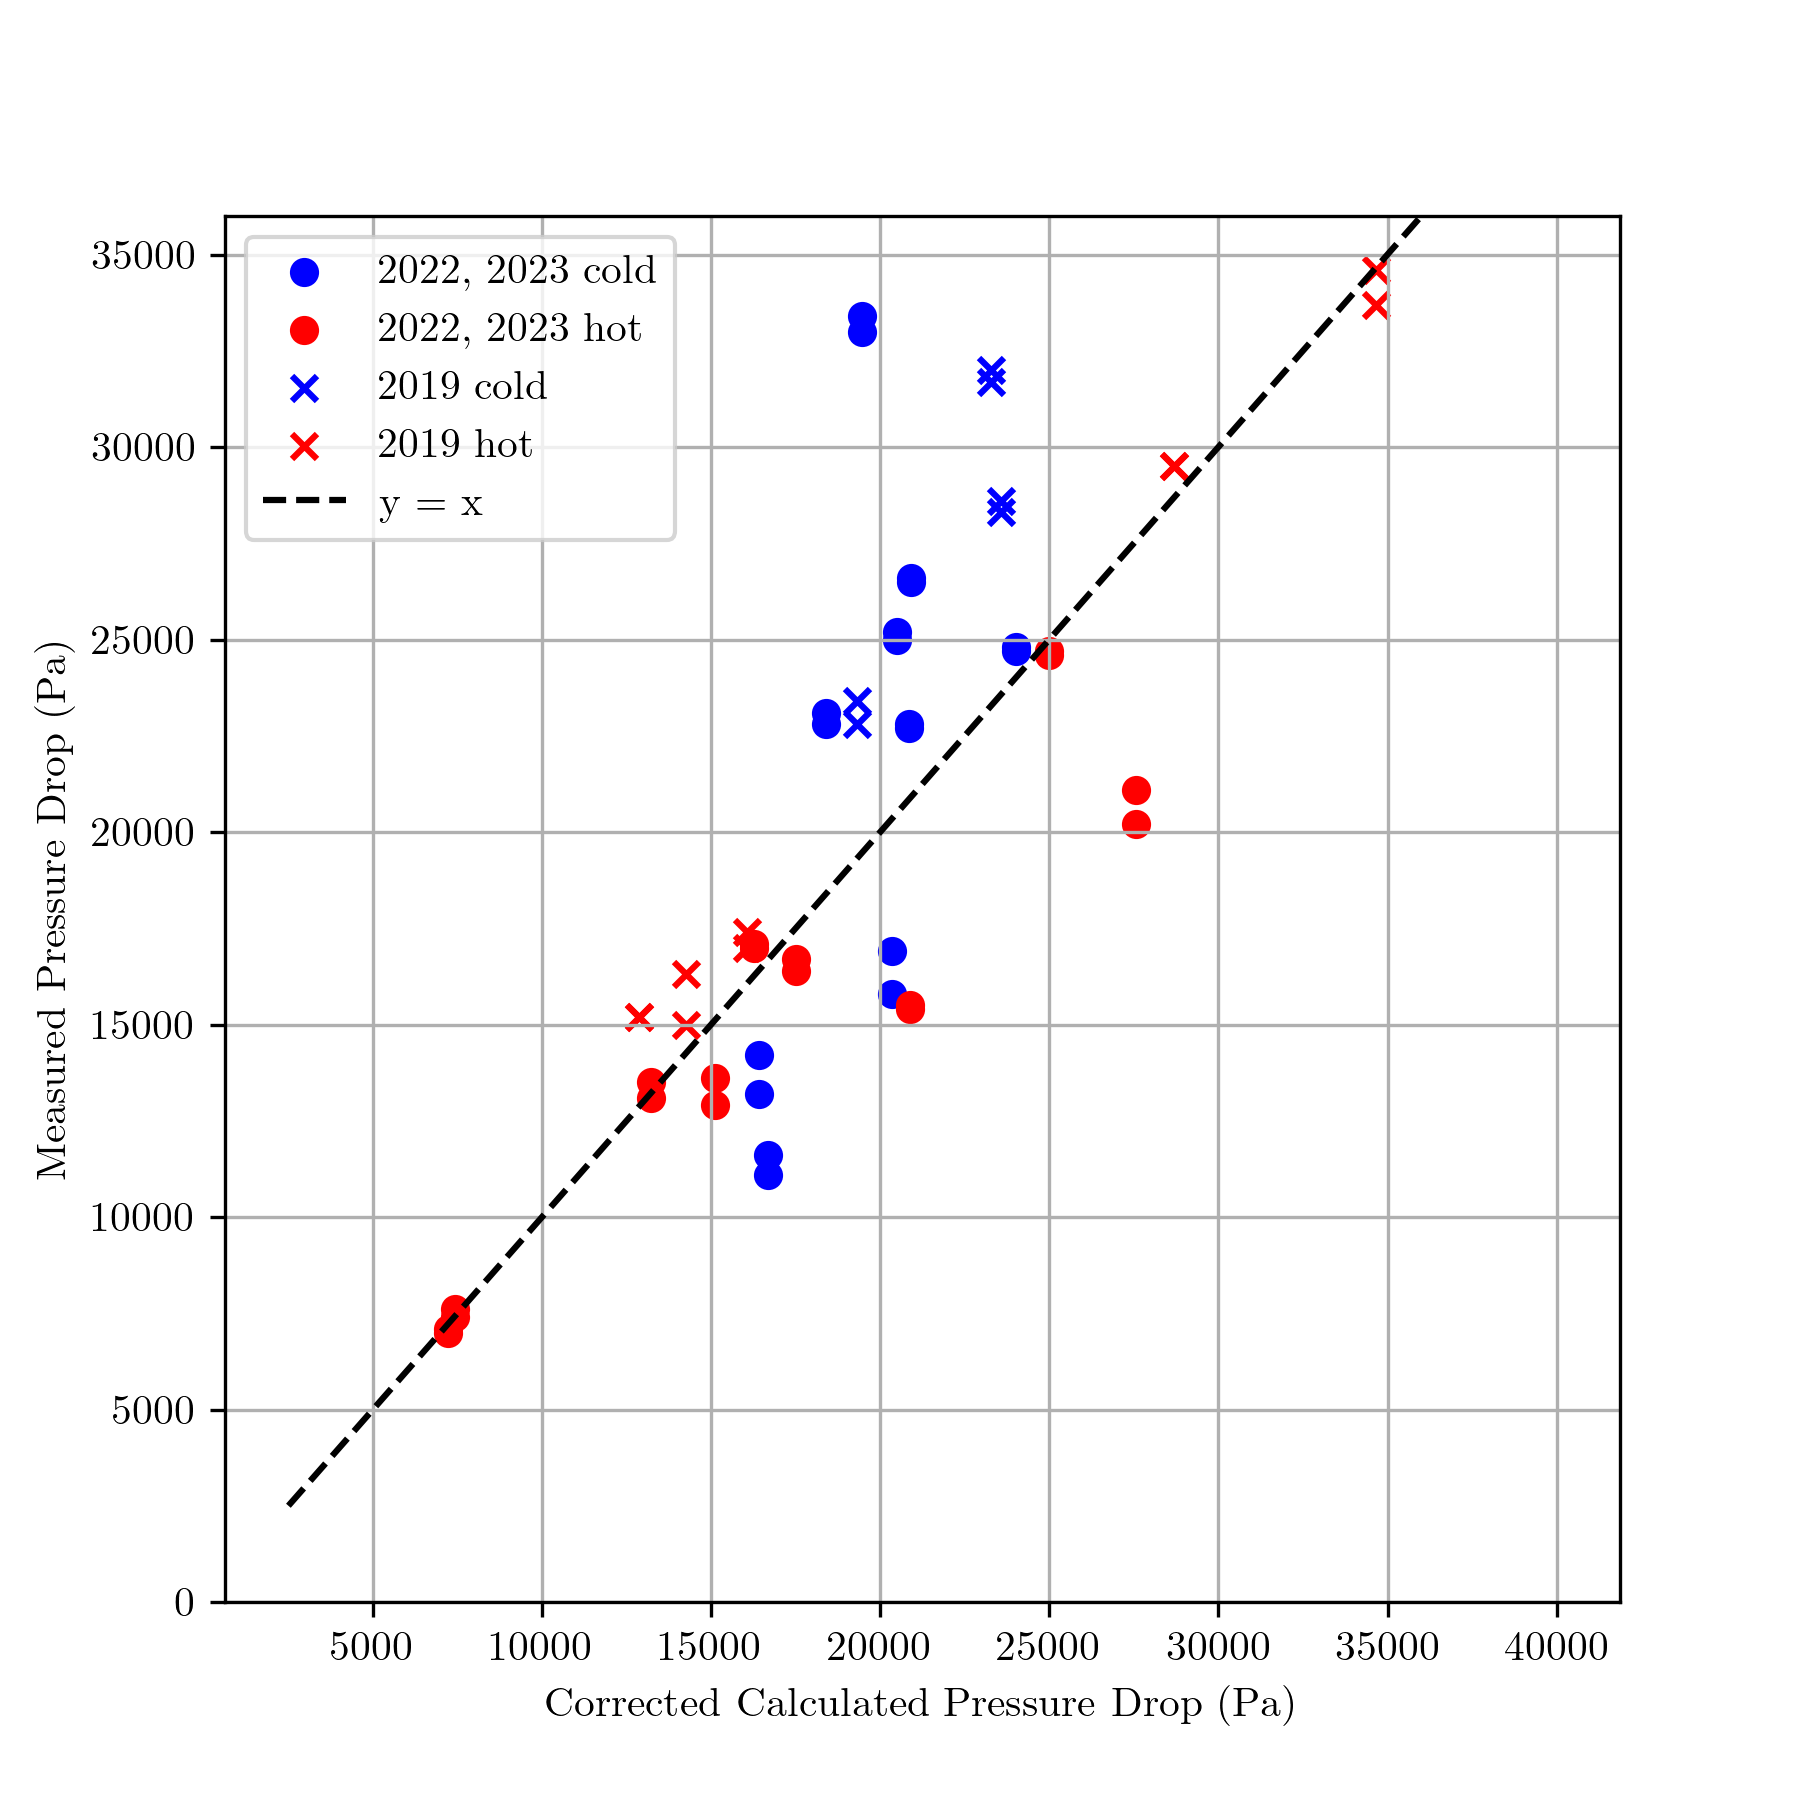
\includegraphics[width=.99\linewidth]{dp_ccalc_vs_meas.png}
    \caption{Applied correction on \ref{fig:uncorrected_pressure_drops} and unseen 2019 designs.}
    \label{fig:corrected_pressure_drops}
  \end{subfigure}
    
  \caption{Pressure drops calculated from measured mass flow rates compared to measured pressure drops.}
  \label{fig:pressure_drops}

\end{figure}

The correlation coefficients for hot and cold pressure drops are $\mathbf{0.93874}$ and $\mathbf{0.50926}$ respectively.
This demonstrates that the model is more accurate at predicting the hot mass flow rate than the cold mass flow rate.
The cold flow pressure drop is generally underestimated by Kerns method, which is expected \cite{HE_design}.
As shown, in the cold flow case, Kerns method significantly underestimates the pressure drop in the cold flow path, and in many cases, outside of the compressor characteristics.
The corrected pressure drop.

\subsubsection{$\mathcal{E}$-NTU and LMTD}


\begin{figure}[H]
  \centering
  \begin{subfigure}{.49\textwidth}
    \centering
    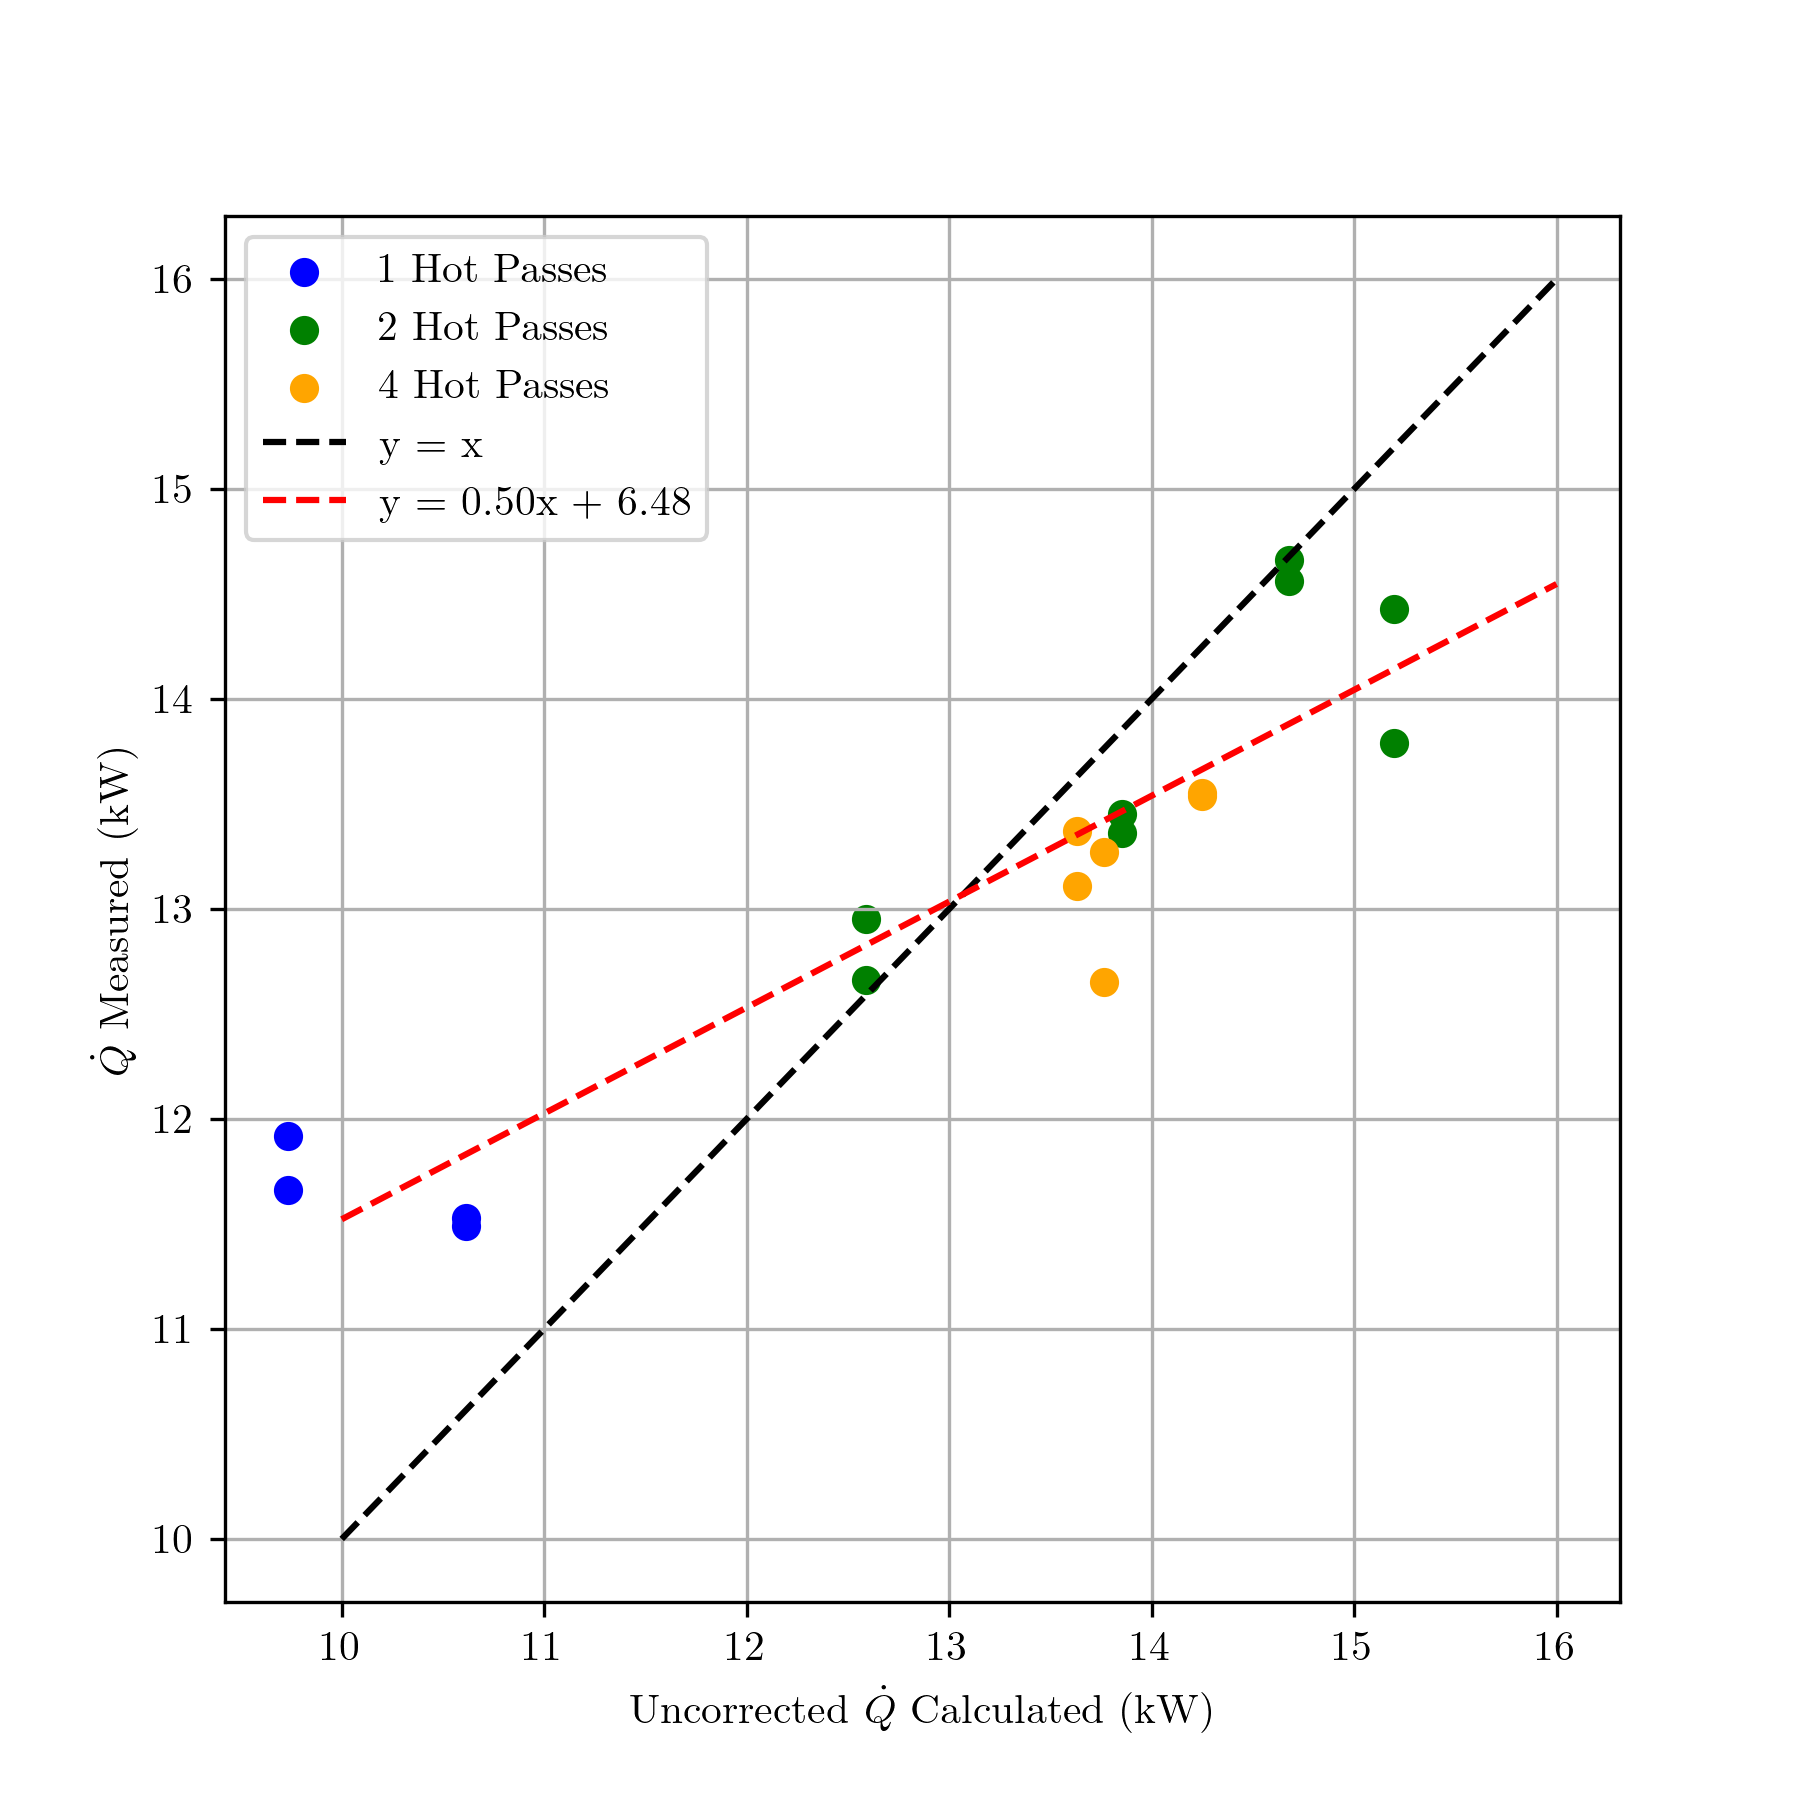
\includegraphics[width=0.99\textwidth]{Qdot_ucalc_vs_measured.png}
    \caption{Correction line from 2022 and 2023 designs.}
    \label{fig:uncorrected_Qdot}
  \end{subfigure}
  \begin{subfigure}{.49\textwidth}
    \centering
    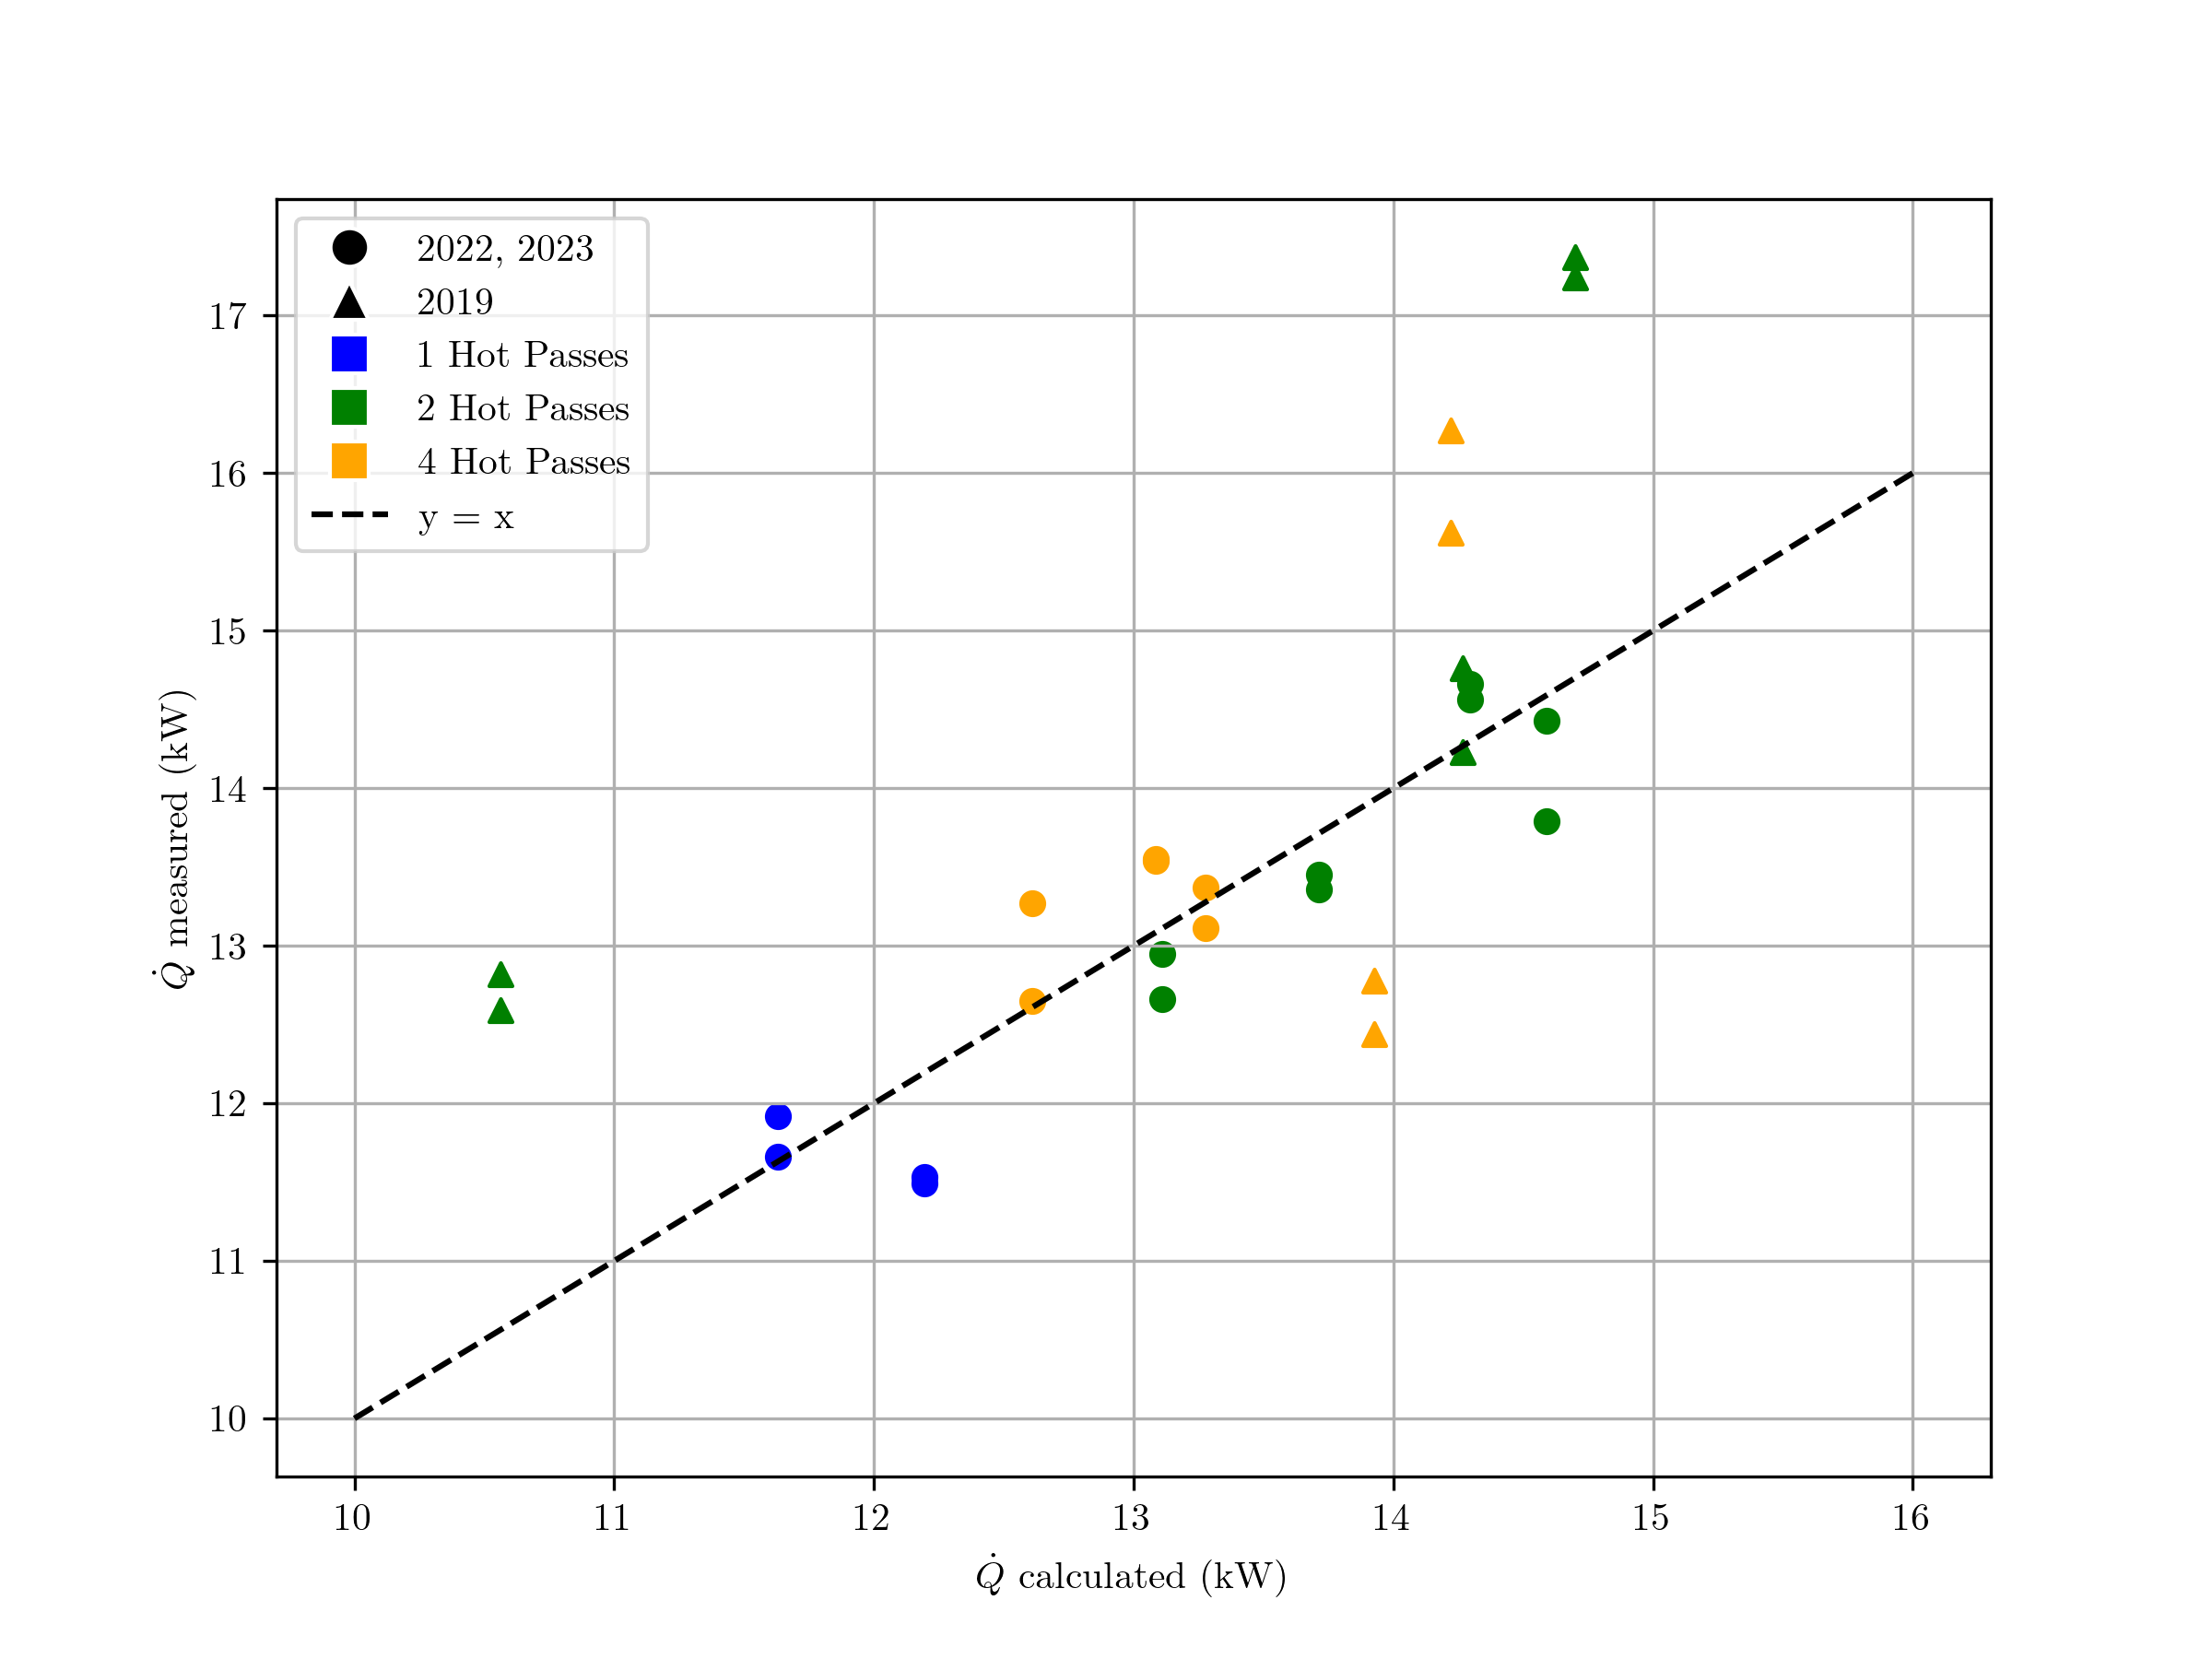
\includegraphics[width=0.99\textwidth]{Qdot_ccalc_vs_measured.png}
    \caption{Applied correction on \ref{fig:uncorrected_Qdot} and unseen 2019 designs.}
    \label{fig:corrected_Qdot}
  \end{subfigure}
  \label{fig:Qdot}
  \caption{Heat transfer rate calculated from measured mass flow rate compared to measured heat transfer rate.}
\end{figure}

\begin{figure}[H]
  \centering
  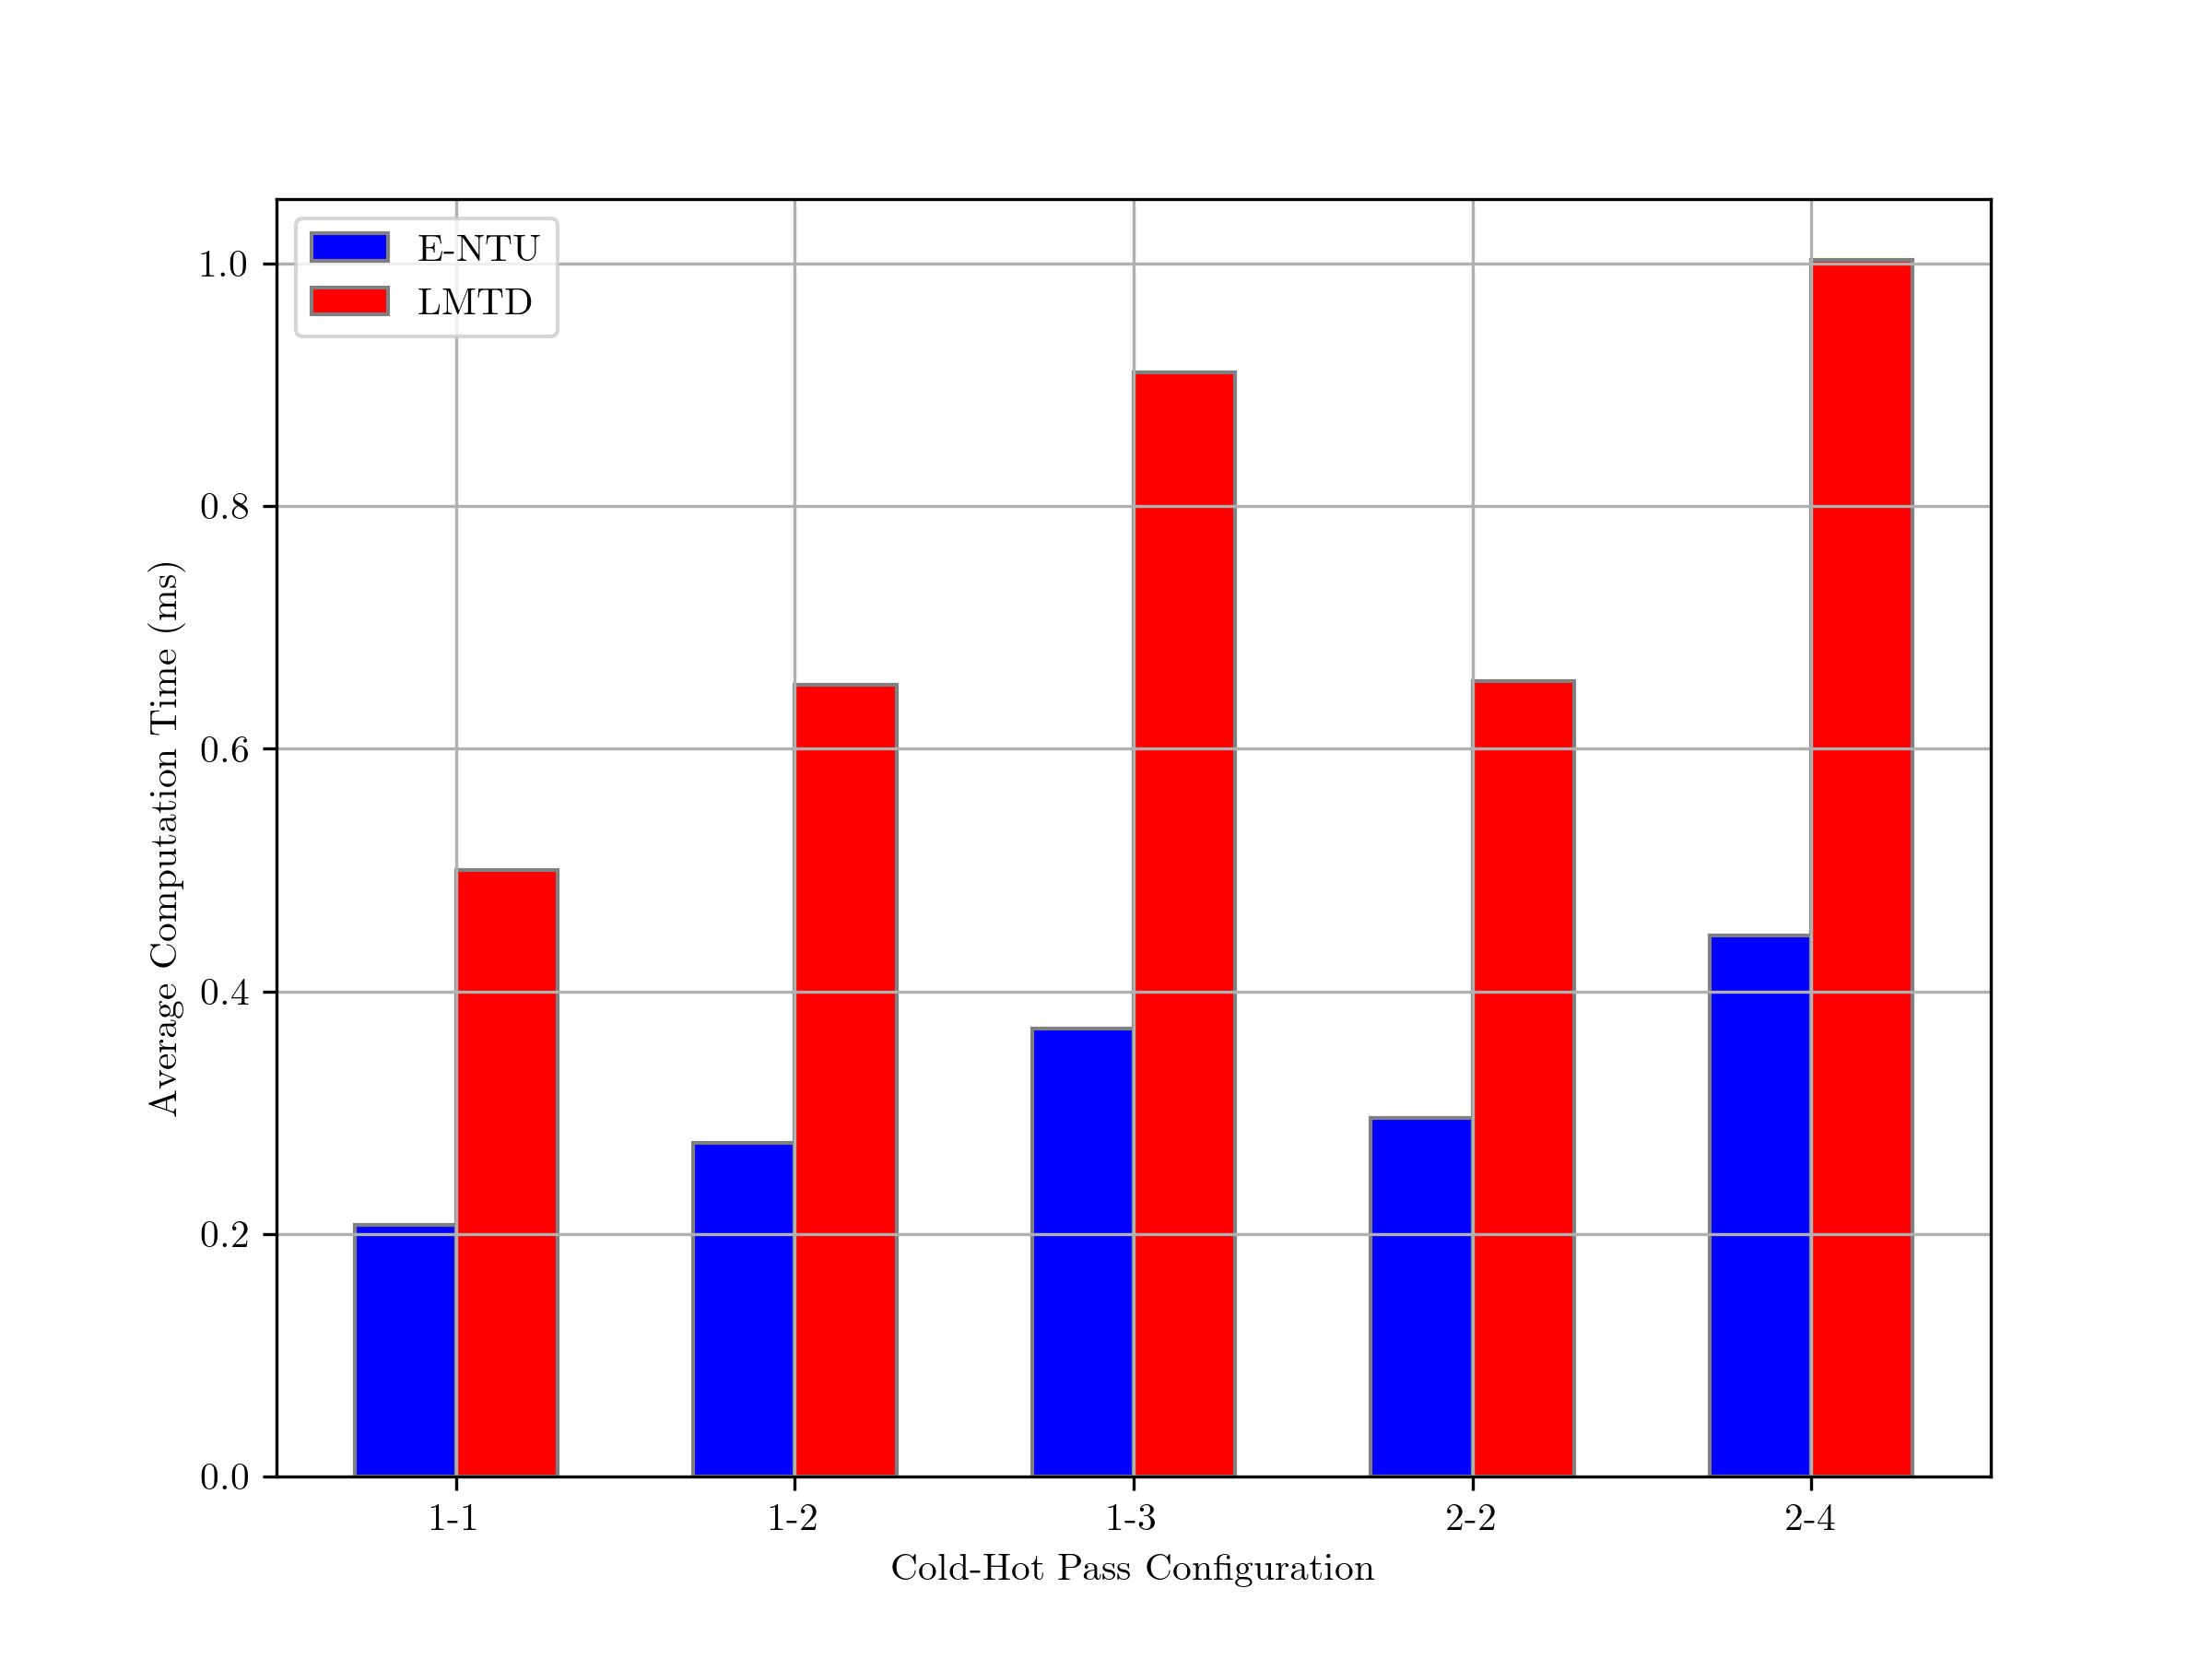
\includegraphics[width=0.6\textwidth]{entu_lmtd_speed.png}
  \caption{Calculation time for $\mathcal{E}$-NTU and LMTD methods for various heat exchanger configurations.}
  \label{fig:entu_lmtd_speed}
\end{figure}

From figure \ref{fig:entu_lmtd_speed} we can see that the $\mathcal{E}$-NTU method is $2$ to $2.5$ times faster than the LMTD method.
This is important for the optimization algorithm as the objective function is calculated thousands of times during the process.


\section{Optimization Problem}

The goal is to maximise the heat transfer rate $\dot{Q}$ subject to physical constraints. For variable flow rate and outlet temperatures, the effectiveness may not be maximised at the maximum heat transfer rate.

\subsection{Constraints}

Many standard physical quantities are constrained to discrete values and standards, such as the number of tubes, baffles and pipe diameters.
For our design, we have the following constraints:
\begin{itemize}
  \item Total mass of the heat exchanger $M < 1.2$ Kg.
  \item Total length of the heat exchanger $L_{\text{total}} < 0.35$ m.
  \item Total length of the tubes $\sum L_{\text{tube}} < 3.5$ m.
  \item Tubes have outer and inner diameters, $d_{o} = 8$ mm, and $d_{i} = 6$ mm.
  \item Shell has inner diameter $D_{\text{shell}} = 64$ mm.
  \item Nozzles must not be closer than $20$ mm to the edge of the shell or header end.
  \item The tube pitch must be greater than $12$ mm.
\end{itemize}

The total length of the tubes constraint must be modified to account for the manufacturing process.
For $n_t$ total tubes, $n_t - 1$ cuts with a blade thickness of $1.5 mm$ are required and so the actual maximum length is given below.
\begin{equation}
  \sum L_\text{tube} < 3.5 - 0.0015 \times (n_t - 1)
\end{equation}
The tube lengths are also limited by the maximum length of the heat exchanger, $0.35$ m.
The nozzle width is 40 mm, however, if there is an even number of hot sections then the nozzles are on the same side so the opposite end section can be shortened.
This can allow a longer maximum tube length than an odd number of hot passes.
\begin{equation}
  L_\text{tube} < 0.29 - 0.02 \times ( N_{hot}\mod 2)
\end{equation}

Additional constraints were also imposed to reduce the search space and simplify the problem.

The number of baffles was constrained to 8 in the cold fluid path. % TODO: explain why this was done other than awais said so

The number of tubes was constrained to not decrease over the hot fluid path inside the heat exchanger.
This should not exclude the global optimium because increasing the area at regions of smaller temperature difference increases overall heat transfer.
For example, if we allowed the area to decrease then more heat transfer would occur in the first stage,
however there would be a significant reduction of heat transfer in the later stages from both reduced area and temperature difference.

\subsection{Design Parameters}

Simplifications were made to reduce the number of design parameters.
For heat exchangers with a large number of tubes, a consistent pattern can be arranged with constant pitch.
However, the nature of this compact design means that the tubes are not arranged in a simple pattern and so the pitch varies between tubes.
It was therefore decided to use an empirical relation to estimate the pitch based on the number of tubes in each equal area hot section.
This assumes that, in each hot flow section, the tubes are packed as far away from each other as possible.
This is assumed to be optimal as it promotes turbulent mixing throughout the shell flow to reduce local temperature gradients.
% Please consider the validity of this assumption

The search space for a given template with $N_\text{hot}$ hot stages and $N_\text{cold}$ cold stages is $(N_\text{hot} + N_\text{cold} + 1)$ dimensional.
This arises from the 1 dimensional length, number of tubes in each hot stage, and number of baffles in each cold stage.
The simplest design has 1 hot stage and 1 cold stage, and so the search space is 3 dimensional.

\subsection{Algorithms}
Three optimization algorithms were tested: Brute force, Sequential Least Squares Programming, and Simplicial Homology Global Optimization.
In an early version of the program, the brute force algorithm was both fast and robust at finding the global optimal design.
However, the introduction of a variable number of tubes and baffles in each stage increased the complexity $O(n^{p+q+1})$.
SLSP was performed for a large number of uniformly distributed random initial values in attempt to find the global optimum.
However, this method required a large number of sample points to find the global optimum and was not robust for the high dimensional search space.

The Simplicial Homology Global Optimization algorithm was chosen for its robustness and ability to find optima in all cases.
SHGO is a derivative-free global optimization algorithm that efficiently subdivides the search space into smaller regions (simplicial complexes) to find the global optimum \cite{SHGO}.

\section{Software}

\subsection{Implementation}

The Python application used PyQt6 and matplotlib for the GUI. The calculations were done using NumPy and SciPy libraries.
The software tool allows the user to interactively change the design parameters for a wide range of heat exchanger configurations.
Calculated values are displayed in real-time and the user can compare the performance of different designs.
When the optimiser is started it will attempt to find the optimal design for the number of stages and tube patterns set.
After an optimal solution is found, the design is loaded into the GUI for manual inspection and comparison with other designs.

\subsection{Design}
The software features object oriented design with classes for the heat exchanger and fluid path components.
The structure is designed to easily modify fluid properties and introduce new flow components.
Seperate optimization threads are used to prevent the GUI from freezing during long calculations.
A log dispays optimization progress, warning and error messages. There is also a diagram of the heat exchanger which helps
the user visualise the flow path of multi-stage designs.

\begin{figure}[H]
  \centering
  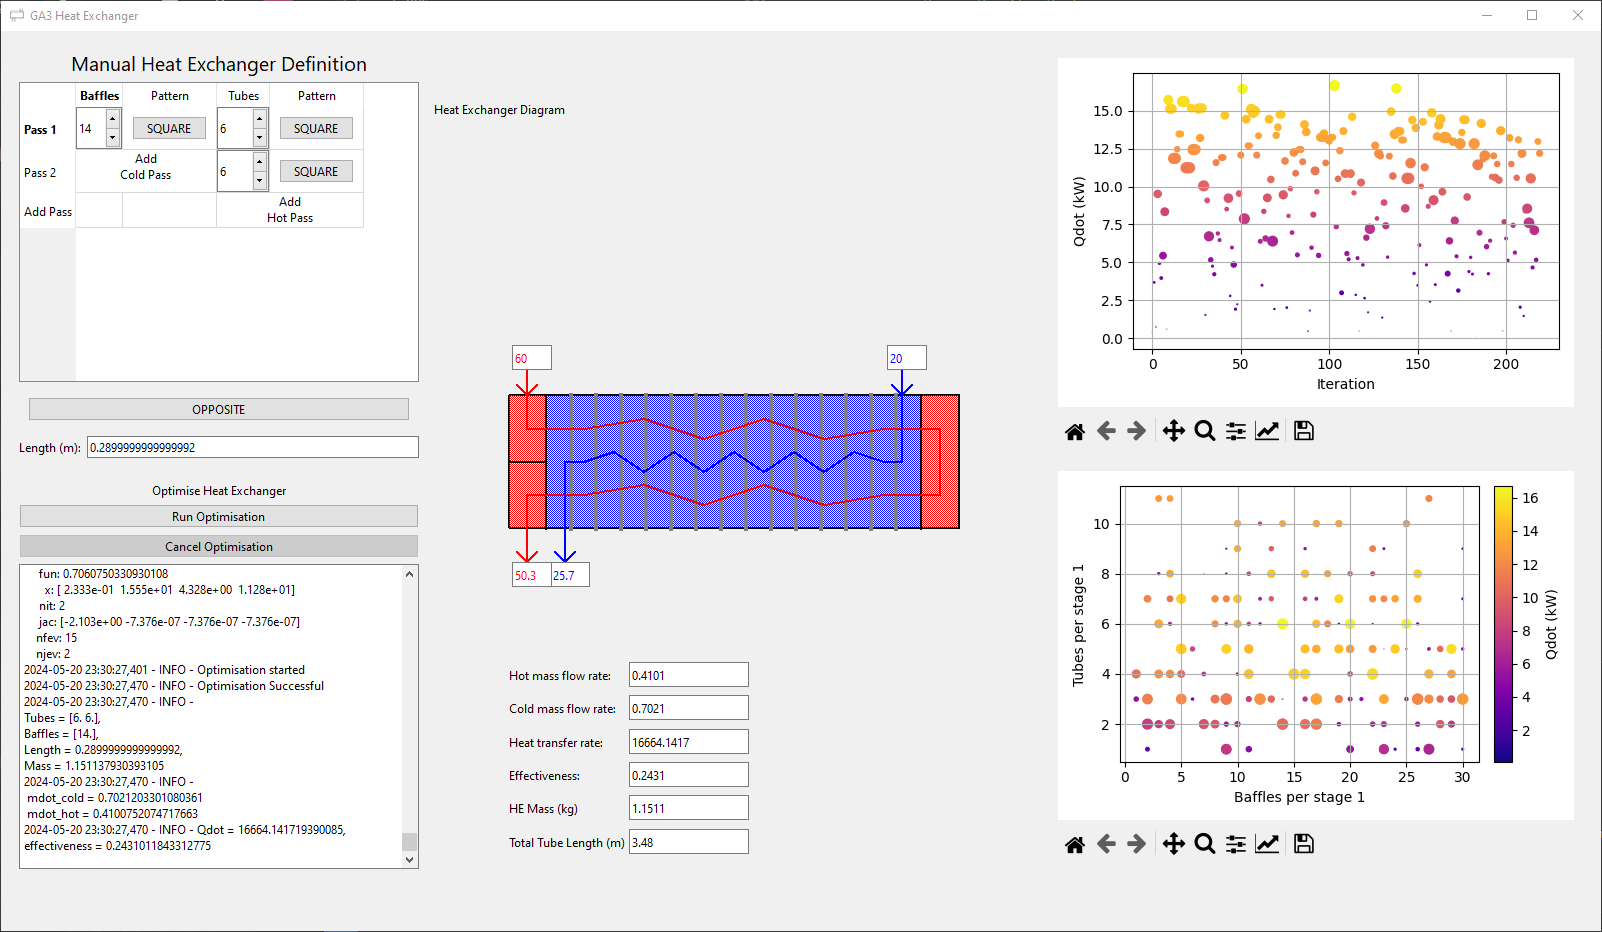
\includegraphics[width=0.6\textwidth]{software.png}
  \caption{Screenshot of the software tool.}
  \label{fig:software}
\end{figure}

\subsection{Best Designs from Constraints}
% challenging to visualise higher dimensional spaces
% I'm not as big as a fan of 3D plots as I used to be - they're harder to interpret than colour maps

\begin{table}[h!]
  \centering
  \begin{tabular}{|c|c|c|c|c|c|c|c|c|c|c|c|}
      \hline
      \rowcolor{gray!30}
      \multicolumn{3}{|c|}{\textbf{Configuration}} & \multicolumn{4}{c|}{\textbf{Optimised Parameters}} & \multicolumn{5}{c|}{\textbf{Result}} \\ \hline
      \rowcolor{gray!10}
      $N_\text{cold}$ & $N_\text{hot}$ & Pattern & Tubes & Baffles & $L_\text{tube}$ & $\dot{m}_1$ & $\dot{m}_2$ & $\dot{Q}$ & $\epsilon$ & Mass & $\Sigma L_\text{tube}$ \\ \hline
      1 & 1 & Triangle & 13 & 8 & 0.2678 & 0.5892 & 0.4778 & 12297 & 0.1446 & 1.095 & \textcolor{red}{3.482} \\ \hline
      1 & 1 & Square & 13 & 8 & 0.2678 & 0.5885 & 0.4778 & 12314 & 0.145 & 1.095 & \textcolor{red}{3.482} \\ \hline
      1 & 2 & Triangle & 6,6 & 8 & 0.2877 & 0.5928 & 0.4296 & 14126 & 0.211 & \textcolor{red}{1.100} & 3.452 \\ \hline
      1 & 2 & Square & 6,6 & 8 & 0.2877 & 0.5928 & 0.4296 & 14123 & 0.2109 & \textcolor{red}{1.100} & 3.452 \\ \hline
      \rowcolor{yellow!60}
      1 & 3 & Triangle & 4,5,5 & 8 & 0.2470 & 0.5818 & 0.3685 & 14328 & 0.2524 & 1.079 & \textcolor{red}{3.481} \\ \hline
      1 & 3 & Square & 5,5,5 & 8 & 0.2320 & 0.5755 & 0.3855 & 14336 & 0.2414 & 1.076 & \textcolor{red}{3.479} \\ \hline
      2 & 2 & Triangle & 5,6 & 8,8 & \textcolor{red}{0.2900} & 0.5908 & 0.4174 & 13896 & 0.2106 & 1.085 & 3.190 \\ \hline
      2 & 2 & Square & 6,6 & 8,7 & 0.2766 & 0.5902 & 0.4304 & 13901 & 0.2044 & \textcolor{red}{1.100} & 3.319 \\ \hline
      2 & 4 & Triangle & 4,4,4,4 & 7,7 & 0.2173 & 0.5714 & 0.3209 & 14136 & 0.2828 & 1.091 & \textcolor{red}{3.478} \\ \hline
      2 & 4 & Square & 4,4,4,4 & 7,7 & 0.2173 & 0.5728 & 0.3209 & 14103 & 0.2816 & 1.091 & \textcolor{red}{3.478} \\ \hline
  \end{tabular}
  \caption{Optimized Designs for a variety of heat exchanger configurations, with the limiting constraint in red.}
  \label{table:designs}
\end{table}

It is important to note that in reality, the pattern of the tubes is not strictly followed in order to fit high numbers of tubes into the heat exchanger.
These arrangements maximise the average pitch and are typically similar to the triangular pattern.
The software overestimates the triangular pitch and underestimates the square pitch to account for this.

It was satisfying to see that the software tool was finding longer solutions with additional tubes in later hot passes over shorter designs with an equal number of tubes in each hot pass.
However, this design with a different number of tubes in each section is much harder to manufacture than a circularly symmetric design.
Manual inspection of the design 

From table \ref{table:designs} the optimal design predicted by the software has 1 cold stage and 3 hot stages.
This was the design that our pair proposed to the group and was selected as the final design configuration.
The circular and axial symmetry in the design was exploited to reduce the number of unique components and simplify the manufacturing process.


\begin{figure}
  \centering
  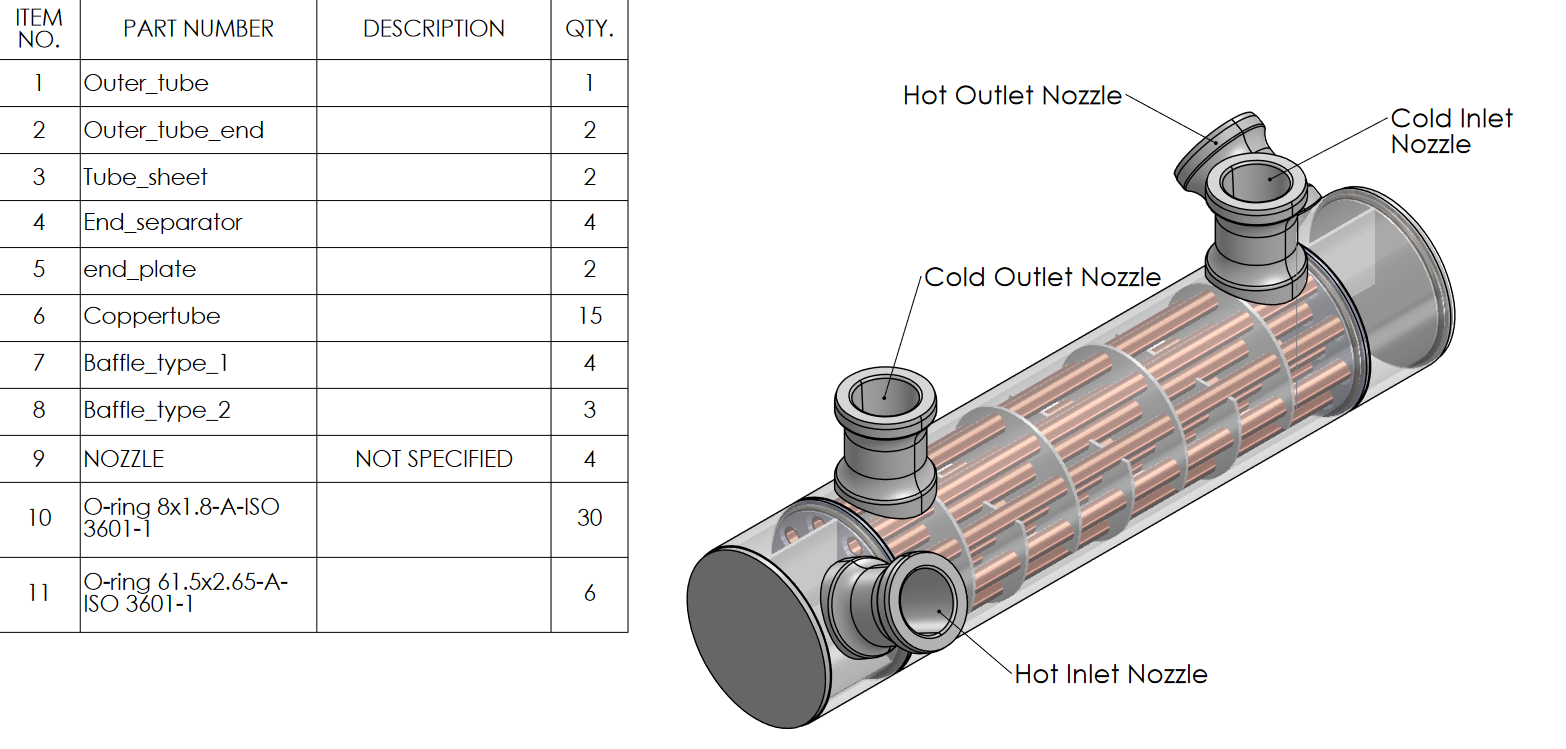
\includegraphics[width=0.7\textwidth]{final.png}
  \caption{Final design parts list with 1 cold stage and 3 hot stages.}
  \label{fig:final_design}
\end{figure}


\begin {lstlisting}[language=Python]

\end{lstlisting}


% bibliography

\begin{thebibliography}{9}

  \bibitem{HeatTransfer}
    Holman J. P.
    \emph{Heat Transfer. 10th ed.}
    McGraw-Hill,
    2010.

%Endres, SC, Sandrock, C, Focke, WW (2018) “A simplicial homology algorithm for lipschitz optimisation”, Journal of Global Optimization.

  \bibitem{handout}
  J. V. Taylor and J. C. Massey
  \emph{GA3 Heat Exchanger Handout}
  University of Cambridge,
  2024.

  \bibitem{worked_example}
  J. V. Taylor and J. C. Massey
  \emph{GA3 Heat Exchanger: Worked Example}
  University of Cambridge,
  2024.

  \bibitem{SHGO}
  Endres, SC, Sandrock, C, Focke, WW,
  \emph{A simplicial homology algorithm for lipschitz optimisation},
  Journal of Global Optimization,
  2018.

  \bibitem{HE_design}
  Sadik Kakac, Hongtan Liu, Anchasa Pramuanjaroenkij,
  \emph{Heat Exchangers: Selection, Rating, and Thermal Design, Third Edition}
  CRC Press,
  2012.

\end{thebibliography}

\end{document}